\documentclass[german,bibliography=totoc]{scrreprt}   
%BCOR8.25mm seht hier bei f�r den abstand von der linken seite, da diese
% gebunden wird
%%%%%%%%%%%%%%%%%%%%%%%%%%%%%%%%%%%%%%%%%%%%%%%%%%%%%%%%%%%%%%%%%%%%%%%%%
%EINGEBUNDENE PAKETE (immer vor dem document ) 
%%%%%%%%%%%%%%%%%%%%%%%%%%%%%%%%%%%%%%%%%%%%%%%%%%%%%%%%%%%%%%%%%%%%%%%%%
\usepackage{bibgerm}			%fuer aufwendigeres literaturverzeichnis mit themes
%\usepackage{amssymb}			% wichtige Symbole
\usepackage{graphics}			% Einbinden von Graphiken
\usepackage[pdftex]{graphicx} 
\usepackage{epstopdf}			%automatischen generieren von pdfs aus eps
\usepackage{array}
\usepackage[centertags]{amsmath} 
\usepackage{amsfonts}			% Schriftart
\usepackage{a4}				% Seitenformat
\usepackage{epsfig}				% Zusaetzliche Graphikbefehle 
\usepackage{floatflt}			% Tabellen
\usepackage{scrpage2}			% useheadings
\usepackage[latin1]{inputenc}	% Umlaute in Windows 
\usepackage{paralist}			% Bessere Enumerate-Umgebungen (Aufzaehlungszeichen
% koennen gewaehlt werden) \usepackage{tabular}			% Tabellen
\usepackage{booktabs}
\usepackage[ngerman,english]{babel}	
\usepackage{mparhack}		% bessere Randnotizen
\usepackage{setspace}		% eigentlich nur fuer den Titel ..
\usepackage{multirow}		% Row-/Columnspan ..
\usepackage{longtable}		%fuer mehrseitige tabellen
\usepackage{makeidx}		%hiermit kann man ein index erstellen, z.b. fuer
% abkuerngen und sozu
\usepackage[T1]{fontenc}	%erweiterter buchstabensatz mit umlauten 
\usepackage{url}			%um URLs darzustellen
\usepackage{thmbox}			%umgebung fuer theoreme und beispiele
\usepackage{color}
\usepackage{xcolor}
\usepackage{caption}
\usepackage{calc}
\usepackage{floatflt}
\usepackage{float}
\usepackage[procnames]{listings}
\usepackage{textcomp}
\usepackage{setspace}
\usepackage{palatino}
% \setlength{\textwidth}{16.5cm}
% \setlength{\evensidemargin}{-0.5cm}
% \setlength{\oddsidemargin}{0.5cm}
% \setlength{\marginparwidth}{18mm}
% \reversemarginpar
% \let\oldmarginpar\marginpar 
% \renewcommand\marginpar[1]{\-\oldmarginpar[\raggedleft\scriptsize #1]%
% {\raggedright\scriptsize #1}}

 %%%%%%%%%%%%%%%%%%%%%%%%%%%%%%%%%%%%%%%%%%%%%%%%%%%%%%%%%%%%%%%%%%%%%%%%%
%COMMANDS 
%%%%%%%%%%%%%%%%%%%%%%%%%%%%%%%%%%%%%%%%%%%%%%%%%%%%%%%%%%%%%%%%%%%%%%%%%%
\renewcommand{\thesubsection}{\Alph{subsection}}
 %%%%%%%%%%%%%%%%%%%%%%%%%%%%%%%%%%%%%%%%%%%%%%%%%%%%%%%%%%%%%%%%%%%%%%%%%
%FORMATIERUNG DES LISTINGS 
%%%%%%%%%%%%%%%%%%%%%%%%%%%%%%%%%%%%%%%%%%%%%%%%%%%%%%%%%%%%%%%%%%%%%%%%%%
\DeclareCaptionFont{white}{\color{white}}
\DeclareCaptionFormat{listing}{\colorbox{gray}{\parbox{\textwidth-2\fboxsep}{#1#2#3}}}
\captionsetup[lstlisting]{format=listing,labelfont=white,textfont=white}
%SMC-Sprache 


%ACCELEO-Sprache
\DeclareCaptionFormat{figure}{\colorbox{gray}{\parbox{\textwidth-2\fboxsep}{#1#2#3}}}
\captionsetup[figure]{format=figure,labelfont=white,textfont=white}

%%%%%%%%%%%%%%%%%%%%%%%%%%%%%%%%%%%%%%%%%%%%%%%%%%%%%%%%%%%%%%%%%%%%%%%%%
%tABELLENFORMATIERUNG
%%%%%%%%%%%%%%%%%%%%%%%%%%%%%%%%%%%%%%%%%%%%%%%%%%%%%%%%%%%%%%%%%%%%%%%%%
%  neuer  Befehl:  \includegraphicstotab[..]{..}
%  Verwendung  analog  wie  \includegraphics
\newlength{\myx}  %  Variable  zum  Speichern  der  Bildbreite
\newlength{\myy}  %  Variable  zum  Speichern  der  Bildh�he
\newcommand\includegraphicsToTab[2][\relax]{%
%  Abspeichern  der  Bildabmessungen
\settowidth{\myx}{\includegraphics[{#1}]{#2}}%
\settoheight{\myy}{\includegraphics[{#1}]{#2}}%
%  das  eigentliche  Einf�gen
\parbox[c][1.1\myy][l]{\myx}{%
\includegraphics[{#1}]{#2}}%
}%  Ende  neuer  Befehl


%%%%%%%%%%%%%%%%%%%%%%%%%%%%%%%%%%%%%%%%%%%%%%%%%%%%%%%%%%%%%%%%%%%%%%%%%
%METAINFORMATIONEN
%%%%%%%%%%%%%%%%%%%%%%%%%%%%%%%%%%%%%%%%%%%%%%%%%%%%%%%%%%%%%%%%%%%%%%%%%
\usepackage[
	pdftitle={Modeling and Simulation Excercises},
	pdfauthor={Alexander Rimer},
	colorlinks=true,
    linkcolor=black,
    citecolor=black,
    filecolor=black,
    pagecolor=black,
    urlcolor=black]{hyperref} %Metainformationen  

%%%%%%%%%%%%%%%%%%%%%%%%%%%%%%%%%%%%%%%%%%%%%%%%%%%%%%%%%%%%%%%%%%%%%%%%%
%SCHRIFT FUER CAPTIONS AENDERN
%%%%%%%%%%%%%%%%%%%%%%%%%%%%%%%%%%%%%%%%%%%%%%%%%%%%%%%%%%%%%%%%%%%%%%%%%
\setkomafont{caption}{\footnotesize \selectfont}
\setkomafont{captionlabel}{\footnotesize \bfseries}
%%%%%%%%%%%%%%%%%%%%%%%%%%%%%%%%%%%%%%%%%%%%%%%%%%%%%%%%%%
%PYTHON HIGHLIGHTING

% Python listing setup
\renewcommand{\lstlistlistingname}{Code Listings}
\renewcommand{\lstlistingname}{Code Listing}
\definecolor{gray}{gray}{0.5}
\definecolor{green}{rgb}{0,0.5,0}
\definecolor{lightgreen}{rgb}{0,0.7,0}
\definecolor{purple}{rgb}{0.5,0,0.5}
\definecolor{darkred}{rgb}{0.5,0,0}
\definecolor{orange}{RGB}{249,124,0}
\definecolor{light_grey_costum}{RGB}{229,229,229}


\lstnewenvironment{python}[1][]{
\lstset{
language=python,
basicstyle=\footnotesize\ttfamily,
stringstyle=\color{green},
showstringspaces=false,
alsoletter={1234567890},
otherkeywords={\ , \}, \{},
keywordstyle=\color{blue},
emph={access,and,as,break,class,continue,def,del,elif,else,%
except,exec,finally,for,from,global,if,import,in,is,%
lambda,not,or,pass,print,raise,return,try,while,assert},
emphstyle=\color{orange}\bfseries,
emph={[2]self},
emphstyle=[2]\color{gray},
emph={[4]ArithmeticError,AssertionError,AttributeError,BaseException,%
DeprecationWarning,EOFError,Ellipsis,EnvironmentError,Exception,%
False,FloatingPointError,FutureWarning,GeneratorExit,IOError,%
ImportError,ImportWarning,IndentationError,IndexError,KeyError,%
KeyboardInterrupt,LookupError,MemoryError,NameError,None,%
NotImplemented,NotImplementedError,OSError,OverflowError,%
PendingDeprecationWarning,ReferenceError,RuntimeError,RuntimeWarning,%
StandardError,StopIteration,SyntaxError,SyntaxWarning,SystemError,%
SystemExit,TabError,True,TypeError,UnboundLocalError,UnicodeDecodeError,%
UnicodeEncodeError,UnicodeError,UnicodeTranslateError,UnicodeWarning,%
UserWarning,ValueError,Warning,ZeroDivisionError,abs,all,any,apply,%
basestring,bool,buffer,callable,chr,classmethod,cmp,coerce,compile,%
complex,copyright,credits,delattr,dict,dir,divmod,enumerate,eval,%
execfile,exit,file,filter,float,frozenset,getattr,globals,hasattr,%
hash,help,hex,id,input,int,intern,isinstance,issubclass,iter,len,%
license,list,locals,long,map,max,min,object,oct,open,ord,pow,property,%
quit,range,raw_input,reduce,reload,repr,reversed,round,set,setattr,%
slice,sorted,staticmethod,str,sum,super,tuple,type,unichr,unicode,%
vars,xrange,zip},
emphstyle=[4]\color{purple}\bfseries,
upquote=true,
morecomment=[s][\color{lightgreen}]{"""}{"""},
commentstyle=\color{red}\slshape,
literate={>>>}{\textbf{\textcolor{darkred}{>{>}>}}}3%
         {...}{{\textcolor{gray}{...}}}3,
procnamekeys={def,class},
procnamestyle=\color{blue}\textbf,
frame=lines,                   	  % angepasst,
numberstyle=\tiny\color{gray},
numbers=left,  
tabsize=2,                      % sets default tabsize to 2 spaces
captionpos=b,                   % sets the caption-position to bottom
breaklines=true,                % sets automatic line breaking
backgroundcolor=\color{light_grey_costum}, %angepasst ende
rulesepcolor=\color{blue},#1
}}{}

 
%%%%%%%%%%%%%%%%%%%%%%%%%%%%%%%%%%%%%%%%%%%%%%%%%%%%%%%%%%

%%%%%%%%%%%%%%%%%%%%%%%%%%%%%%%%%%%%%%%%%%%%%%%%%%%%%%%%%%%%%%%%%%%%%%%%%
%DOKUMENT BEGINN
%%%%%%%%%%%%%%%%%%%%%%%%%%%%%%%%%%%%%%%%%%%%%%%%%%%%%%%%%%%%%%%%%%%%%%%%%
\begin{document}  
\setcounter{chapter}{1}
 

%Die Uebungen    
%Title 
\begin{figure}
\centering
{\Huge Model Building and Simulation (MODUS)}\\[0.5cm]
{\Huge Exercise 3}\\[0.5cm]
{\Large Alexander Rimer / Eleni Milona}\\[0.6cm]  
{\Large 1138243 / 1150221}\\[0.6cm]  
\today
\end{figure}

\section{Modeling the realworld problems}
\subsection{Patient transport logistics (PTL)}
Following sequence diagram describes the first scenario: 
\begin{figure}[!htb]
  \centering   
  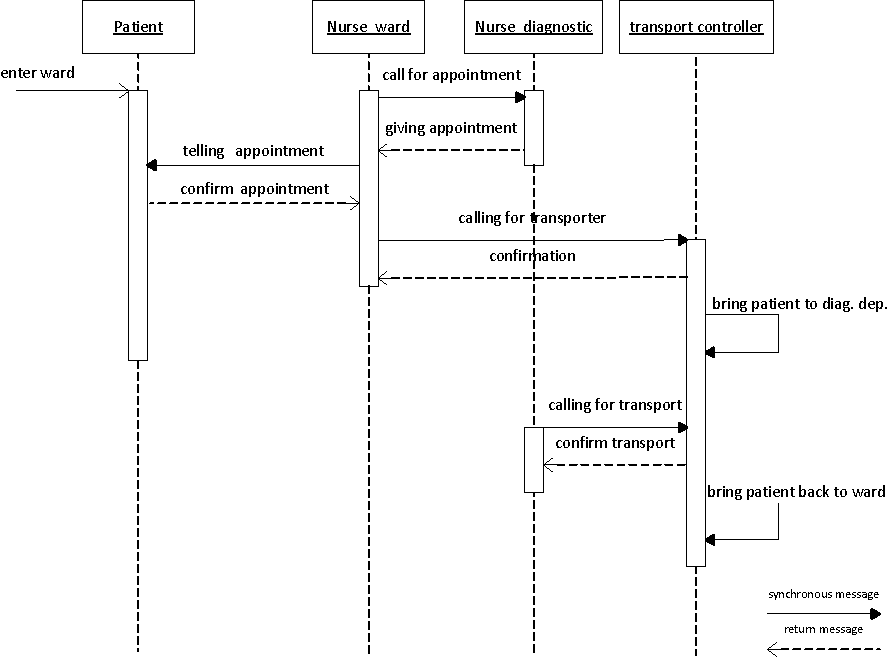
\includegraphics[width=1\textwidth]{pics/ub3/a/1a_seq} 
  \caption{Sequence diagram for scenario 1}
  \label{fig:1a_seq_dia} 
 \end{figure}
\newpage

\textbf{Statechart for patient:}
\begin{figure}[!htb]
  \centering  
  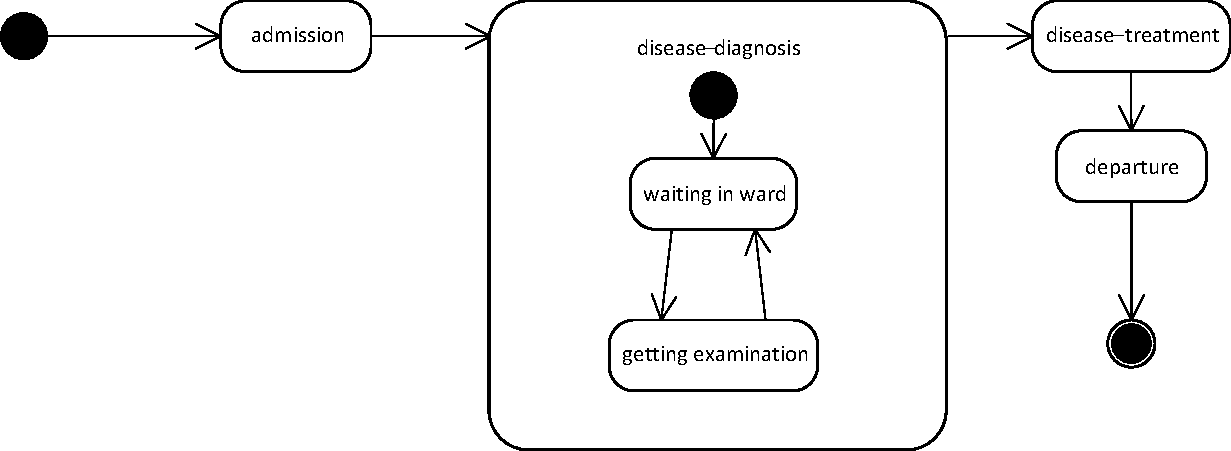
\includegraphics[width=1\textwidth]{pics/ub3/a/1a_pat} 
  \caption{Statediagram for patient}
  \label{fig:1a_pat_dia} 
 \end{figure}
 
\textbf{Statechart for nurses (ward/diagnostic):}
\begin{figure}[!htb]
  \centering  
  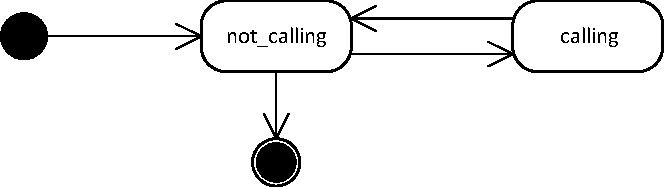
\includegraphics[width=0.7\textwidth]{pics/ub3/a/1a_nurse} 
  \caption{Statediagram for nurses}
  \label{fig:1a_nurse_dia} 
 \end{figure}
 
 \textbf{Statechart for transport controller:}
\begin{figure}[!htb]
  \centering  
  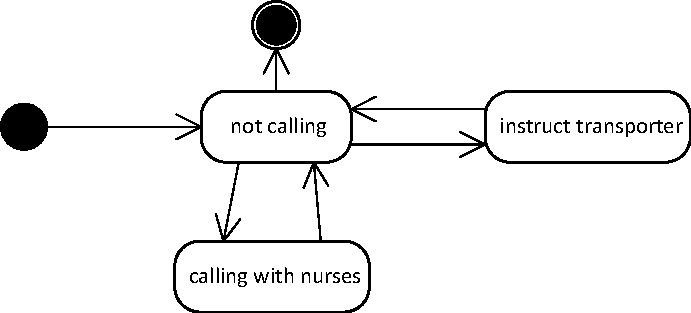
\includegraphics[width=0.7\textwidth]{pics/ub3/a/1a_contr} 
  \caption{Statediagram for transport controller}
  \label{fig:1a_contr_dia} 
 \end{figure}
 
 
 \newpage
\subsection{OP PEP}
Following sequence diagram describes the second scenario:
\begin{figure}[!htb]
  \centering  
  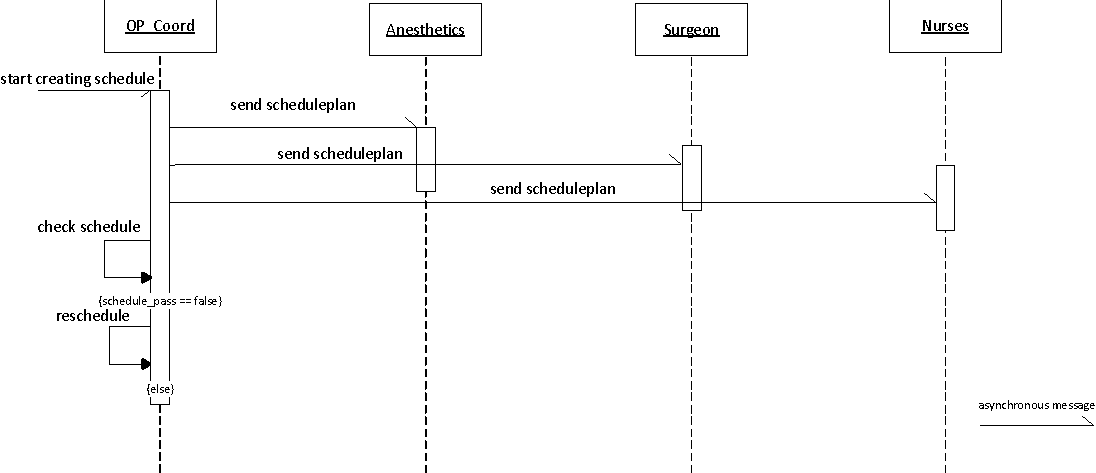
\includegraphics[width=1.1\textwidth]{pics/ub3/b/1b_seq} 
  \caption{Sequence diagram for scenario 2}
  \label{fig:1b_seq} 
 \end{figure}
 
 \textbf{Statechart for OP coordinator:}
\begin{figure}[!htb]
  \centering  
  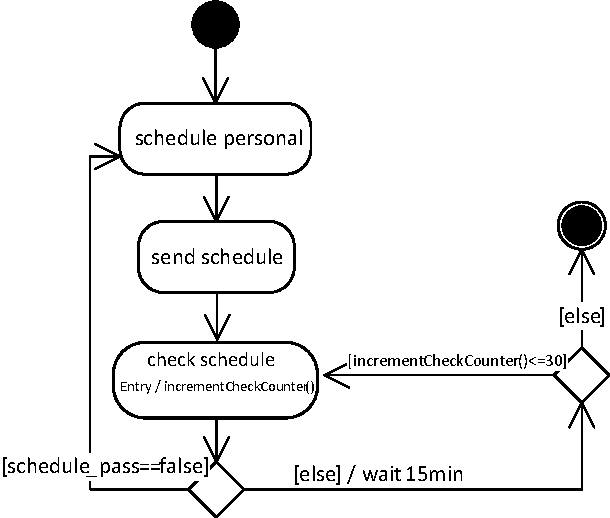
\includegraphics[width=0.7\textwidth]{pics/ub3/b/1b_orga_stat} 
  \caption{Statediagram for coordinator}
  \label{fig:1b_orga_stat} 
 \end{figure}
 
 \newpage
 
  \textbf{Statechart for surgeon:}
\begin{figure}[!htb]
  \centering  
  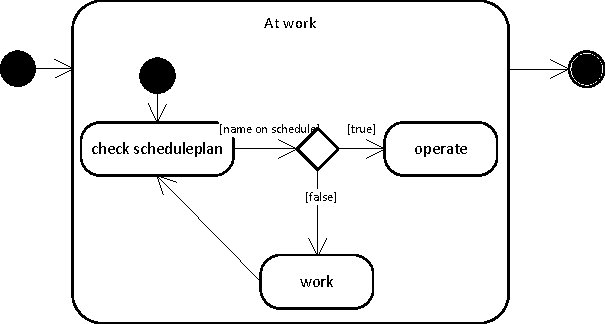
\includegraphics[width=0.7\textwidth]{pics/ub3/b/1b_chir_stat} 
  \caption{Statediagram for surgeon}
  \label{fig:1b_chir_stat} 
 \end{figure}
 
   \textbf{Statechart for anesthetist:}
\begin{figure}[!htb]
  \centering  
  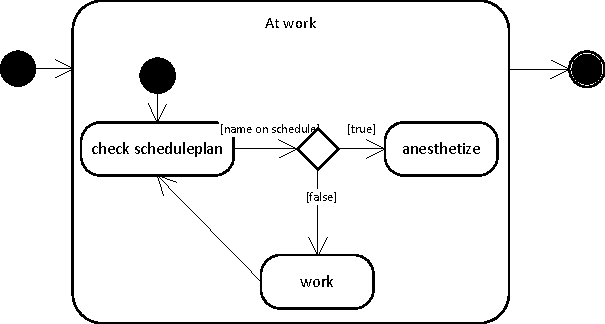
\includegraphics[width=0.7\textwidth]{pics/ub3/b/1b_anest_stat} 
  \caption{Statediagram for anesthetist}
  \label{fig:1b_anest_stat} 
 \end{figure}
 
 
    \textbf{Statechart for nurse:}
\begin{figure}[!htb]
  \centering  
  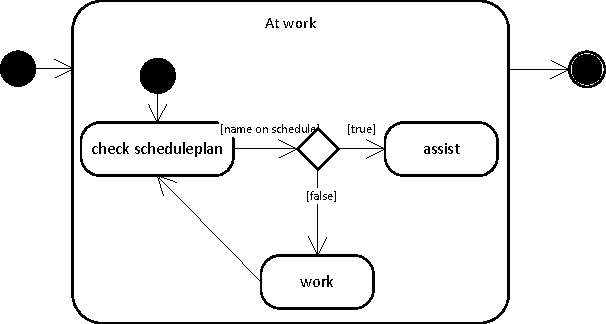
\includegraphics[width=0.7\textwidth]{pics/ub3/b/1b_nurse_stat} 
  \caption{Statediagram for nurse}
  \label{fig:1b_nurse_stat} 
 \end{figure}

\newpage 
\textbf{Whole statechart for patient:}
\begin{figure}[!htb]
  \centering  
  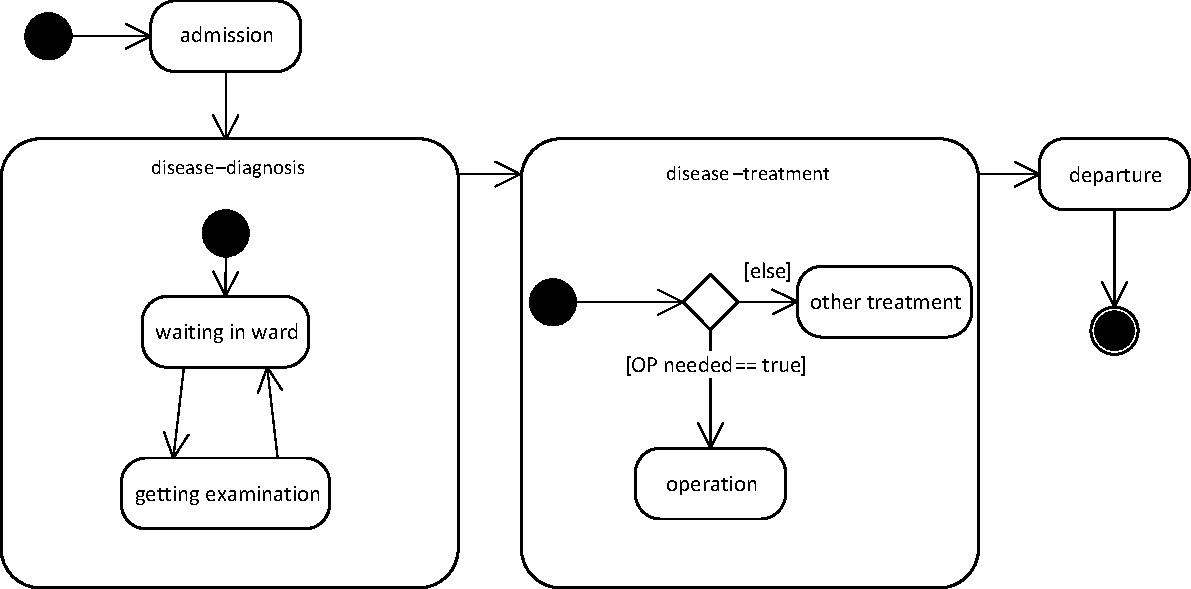
\includegraphics[width=1\textwidth]{pics/ub3/b/1b_pat_stat} 
  \caption{Statediagram for patient}
  \label{fig:1b_pat_stat} 
 \end{figure}
 


 



\end{document}
